\section{Work Plan}

The following section describes the approach taken by the FANS development team to collaborate effectively and complete
the FANS system before its deadline.

\subsection{The Project Team}

Each member of the project team is a third year computer systems engineering student.

\textbf{Grant Achuzia} \\
Grant's strengths lie in effective project management and organization, and he is passionate about delivering successful
projects in academic settings. Grant also has significant experience designing web interfaces that are accessible and
aesthetically pleasing.

\textbf{Matteo Golin} \\
Matteo has background in developing embedded system on Raspberry Pi's from his work at Carleton University's rocketry
design team, where he is leading the development of a real-time telemetry system using Blackberry's QNX RTOS.

\textbf{Saja Fawagreh} \\
Saja has developed skills in user interface design from her time on co-op, and excels and making visually appealing
interfaces because of her sharp attention to detail.

\textbf{Javeria Sohail} \\
Javeria has expertise in system architecture design, and has a strong knowledge of object-oriented design patterns. She
is passionate about optimization, efficient design and modularity.

\subsubsection{Roles and Tasks}

\begin{table}[H]
    \centering
    \begin{tabular}{| c | p{3cm} | p{4cm} | p{5cm} |}
        \hline
        \textbf{Team Member} & \textbf{Major Role/Task (Primary)} & \textbf{Secondary Responsibility (Testing)} &
        \textbf{Reason for assignment}                                                                                                  \\
        \hline
        Grant Achuzia        & User interface design              & Local network communication                 & Very
        familiar with HTML/CSS/JavaScript and has knowledge of good web design practices.                                               \\
        \hline
        Matteo Golin         & Sensor data collection             & Local network communication                 &
        Experience writing software to drive sensors and collect data from them because of his experience with CU
        InSpace. Familiar with networking protocols from 5G automation co-op at DELL Technologies.                                      \\
        \hline
        Saja Fawagreh        & Notification system                & Local network communication                 &
        Good communicator, capable of writing succinct Python logic for accomplishing the task.                                         \\
        \hline
        Javeria Sohail       & Haptic alarm system                & Local network communication                 & Familiar with LED and
        buzzer actuators from SYSC3310.                                                                                                 \\
        \hline
    \end{tabular}
    \caption{Assignment of team members to major project tasks}
\end{table}

\subsubsection{Teamwork Strategy}

\textbf{Regular Team Meetings} \\
We will schedule regular team meetings to discuss project progress, share updates, and address any challenges or
questions. Our team will establish MS Teams as our main communication channel to ensure efficient communication within
the team and with the TA.

Additionally, the team meetings will be documented to review what we talked about in the case that someone misses a
meeting.

\textbf{Version Control} \\
We will use GitHub to manage our codebase changes. This will include practices such as creating branches for features or bug
fixes, committing regularly, and requiring code reviews before merging pull requests.

Informative commit messages that follow the SYSC3010 commit formatting guidelines will be required to avoid
misunderstandings.

The team will release frequent prototypes using GitHub's version release features. Versioning will follow
\textit{semantic versioning} (semver) notation. \cite{semver}

\textbf{Code Reviews} \\
Before merging code changes, thorough code reviews will be conducted to ensure code quality and maintainability, as well
as gain feedback about feature implementations from other team members.

\textbf{Testing} \\
We will follow a testing strategy that includes unit testing, integration testing, and system testing to ensure the
reliability and robustness of the FANS.

FANS will be frequently prototyped to ensure a working system at each development step. This methodology is in
accordance with the V-model. \cite{v-model} To ensure this, mocking will be used to simulate modules of the system that
haven't been fully implemented.

Unit testing will be written by developers who have written the feature under test, and will also be run as GitHub
workflows on pull requests to ensure that new code does not break existing functionality.

\textbf{Feedback} \\
Team members will provide constructive feedback to each other for continuous improvement and learning (also making use
of Feedback Fruits). We will also request feedback from our TA at every milestone so that our final system comes together
seamlessly.

\subsubsection{What We Will Need to Learn}

\textbf{Hardware integration} \\
Since the FANS includes both hardware and software components, we need to learn how to integrate them seamlessly. We
utilize online resources and forums where hardware integration techniques are discussed. Many of our hardware modules
(SenseHat, AudioHat, etc.) have associated online tutorials and a plethora of information associated with them.
\cite{sensehat} We will leverage this information.

\textbf{Real-time communication} \\
Implementing real-time communication features such as SMS and email notifications requires
knowledge of APIs and protocols for sending messages. We will look at the documentation and instructions provided by
communication service providers (e.g. SMS) and learn how to integrate these services into our system.

We will also seek out Python tutorials for automated email sending, as there are several Python libraries that provide
this functionality (such as \texttt{smtplib} \cite{python-email}).

\textbf{Developing a web interface} \\
Creating a user-friendly web interface for the FANS requires knowledge of front-end development, including HTML, CSS
and JavaScript. We will use online tutorials, courses and documentation of web development frameworks such as React.

\textbf{Test strategies} \\
Developing effective testing strategies, including unit testing, integration testing, and system
testing, requires an understanding of various testing frameworks and methodologies. We will explore tutorials for
language specific testing frameworks, and use online resources to teach ourselves how to effectively mock components of
our system.

\subsection{Project Milestones}

\begin{table}[H]
    \centering
    \begin{tabular}{| c | c | p{9cm} |}
        \hline
        \textbf{Milestone Name} & \textbf{Date} & \textbf{Description}                                                                            \\
        \hline
        UI                      & 2024-02-25    & Develop a user-friendly web interface for monitoring system status, configuring thresholds, and
        interacting with the system.                                                                                                              \\
        \hline Database         & 2024-02-28    & Set up a database to store employee contact information
        and system data, ensuring efficient management and retrieval.                                                                             \\
        \hline
        Sensor integration      & 2024-03-05    & Integrate sensors with the Raspberry Pi for real-time data collection, enabling the
        system to monitor environmental conditions.                                                                                               \\
        \hline Smoke detection  & 2024-03-13    & Develop and test
        the smoke detection algorithm on the Raspberry Pi to ensure accurate detection of fire and smoke.                                         \\
        \hline
        Notifications           & 2024-03-19    & Implement a notification system to trigger alarms and alert users via SMS and email
        in case of fire emergencies.                                                                                                              \\
        \hline
        Testing                 & 2024-03-27    & Conduct comprehensive testing to ensure the functionality and integration of both
        hardware and software components.                                                                                                         \\
        \hline
        Finalization            & 2024-03-30    & Finalize system configuration, including thresholds and notification settings, and
        conduct comprehensive testing.                                                                                                            \\
        \hline
    \end{tabular}
    \caption{Major milestones for FANS development.}
\end{table}

\subsection{Schedule of Activities}

\begin{figure}[H]
    \centering
    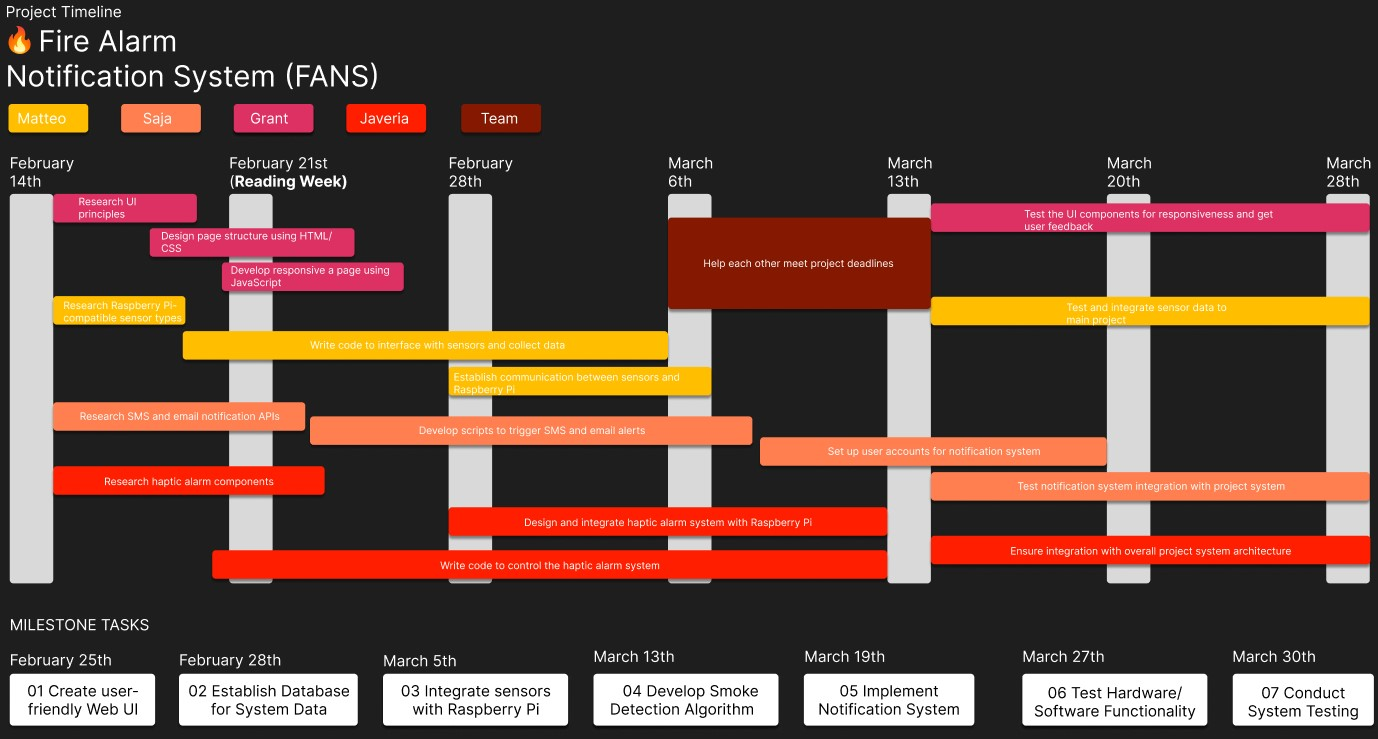
\includegraphics[width=\linewidth]{../assets/SYSC3010_ProjectTimeline.jpg}
    \caption{Project Timeline for Group L1-G8}
\end{figure}
